\documentclass[12pt,a4paper]{article}
\usepackage[utf8]{inputenc}
\usepackage[T1]{fontenc}
\usepackage[english]{babel}
\usepackage{amsmath,amssymb,amsfonts,mathtools}
\usepackage{geometry}
\geometry{left=2cm,right=2cm,top=2cm,bottom=2cm}
\usepackage{booktabs}
\usepackage{hyperref}
\usepackage{url}
\usepackage{graphicx}
\usepackage{caption}
\usepackage{subcaption}
\usepackage{float}
\usepackage{siunitx}
\usepackage{bm}
\usepackage{pgfplots}
\pgfplotsset{compat=1.18}
\usepackage{xcolor}
\usepackage{multicol}
\usepackage{fontspec}
\setmainfont{Calibri}
\setsansfont{Segoe UI}[BoldFont=Segoe UI Bold, Ligatures=TeX]
\usepackage{tikz}
\usetikzlibrary{positioning, arrows.meta, calc}

\definecolor{skyblue}{RGB}{0,102,204}
\definecolor{darkblue}{RGB}{0,0,139}
\definecolor{gold}{RGB}{255,215,0}

% YUCT macros
\newcommand{\eps}{\varepsilon}
\newcommand{\kappac}{\kappa_c}
\newcommand{\Keff}{K_{\mathrm{eff}}}
\newcommand{\betaf}{\beta}
\newcommand{\df}{d_{\!f}}
\newcommand{\Mpl}{M_{\mathrm{Pl}}}
\newcommand{\Lpl}{l_{\mathrm{Pl}}}
\newcommand{\tP}{t_{\mathrm{P}}}
\newcommand{\Sodd}{S_{\mathrm{odd}}}
\newcommand{\Seven}{S_{\mathrm{even}}}
\newcommand{\Dtau}{\Delta\tau_{\min}}
\newcommand{\Lzero}{L_0}
\newcommand{\Omegarot}{\Omega_{\mathrm{rot}}}
\newcommand{\Mbar}{M_{\mathrm{bar}}}
\newcommand{\muniv}{M_{\mathrm{univ}}}

\title{\textbf{YUCT Critical Mass and Cosmic Hierarchy: A Self-Contained Summary for Human and AI Readers}}
\author{Alexey V. Yakushev}
\date{April 2026}

\begin{document}
	\maketitle
	
	\begin{abstract}
		This document provides a concise, self-contained summary of key results from the Yakushev Unified Coordination Theory (YUCT) concerning the critical mass of a local Big Bang, the associated inflationary parameters, the global rotation of the Universe, and the cosmic mass hierarchy. All equations are explicitly marked as YUCT relations. The document is structured for easy ingestion by both human readers and AI language models, with clear formulas, tables, and falsifiable predictions. A complete hierarchy of masses from the Planck scale to the observable Universe is presented, demonstrating the unification of quantum, stellar, and cosmological scales through a single coordination scaling law.
	\end{abstract}
	
	\section{Fundamental Postulates of YUCT}
	
	\begin{itemize}
		\item \textbf{Coordination efficiency} (YPSDC protocol, Appendix B):
		\[
		\Keff = \frac{H(\mathcal{A})}{H(\kappa)}, \qquad\text{(YUCT-1)}
		\]
		where \(H(\mathcal{A})\) is the entropy of the activated action and \(H(\kappa)\) is the entropy of the transmitted short index.
		
		\item \textbf{Universal error scaling law} (Appendix L):
		\[
		\varepsilon = \kappac \alpha \Keff^{-\betaf}, \qquad \betaf = \frac{2}{3},\ \kappac = \frac{1}{3}. \qquad\text{(YUCT-2)}
		\]
		
		\item \textbf{Algebraic loop} (Appendix Y):
		\[
		\Sodd = \frac{6}{5},\quad \Seven = \frac{4}{5},\quad \frac{\Sodd}{\Seven} = \frac{3}{2} = \frac{1}{\betaf}. \qquad\text{(YUCT-3)}
		\]
		Fundamental length and time quanta:
		\[
		\Lzero = \frac{2}{3}\Lpl,\qquad \Dtau = \frac{2}{3}\tP. \qquad\text{(YUCT-4)}
		\]
		
		\item \textbf{Fractal dimension} from information saturation (Appendix L):
		\[
		d_f = \frac{11}{5}=2.2. \qquad\text{(YUCT-5)}
		\]
	\end{itemize}
	
	\section{Critical Mass of a Local Big Bang}
	
	Using the scaling law derived from the consistency of the coordination network,
	\[
	\Keff(R) = \left(\frac{R}{\Lzero}\right)^{\betaf d_f/2}, \qquad\text{(YUCT-6)}
	\]
	and the critical condition \(\varepsilon \approx 1\) (i.e., \(\Keff = K_{\mathrm{crit}} = 3^{3/2}\)), one obtains the critical mass of a gravitationally bound pre‑collapse region:
	\[
	M_{\mathrm{crit}} = 3 M_{\mathrm{Pl}} \approx 6.5\times 10^{-8}\ \mathrm{kg}. \qquad\text{(YUCT-7)}
	\]
	The derivation uses the Schwarzschild radius \(R_S = 2GM/c^2\) and the algebraic loop \(\Lzero = \frac{2}{3}\Lpl\). Quantum corrections leave the coefficient 3 unchanged at leading order.
	
	\section{Cosmological Inflation as a Coordination Phase Transition}
	
	The inflationary observables are predicted from the same postulates:
	\begin{align}
		n_s &= 1 - 2\betaf^2 + \frac{4}{3}\betaf^3 + \cdots \approx 0.965, \qquad\text{(YUCT-8)}\\
		r &= 8(2\betaf)^2 = 32\betaf^2 \approx 0.07, \qquad\text{(YUCT-9)}\\
		f_{\mathrm{NL}}^{\mathrm{local}} &= \frac{5}{3}\betaf \approx 1.12. \qquad\text{(YUCT-10)}
	\end{align}
	These predictions are falsifiable by CMB‑S4, LiteBIRD, Euclid, and SPHEREx.
	
	\section{Global Rotation of the Universe}
	
	The CMB dipole is partially due to a global, rigid rotation with angular velocity \(\omega\). The dipole amplitude grows with redshift \(z\) as:
	\[
	v_{\mathrm{dip}}(z) = v_{\mathrm{local}} + \omega\, r(z). \qquad\text{(YUCT-11)}
	\]
	From the growth observed in NVSS, Quaia, and other surveys, one obtains
	\[
	\omega \approx 8.5\times 10^{-22}\ \mathrm{rad/s},\qquad
	T_{\mathrm{rot}} = \frac{2\pi}{\omega} \approx 2.3\times 10^{14}\ \mathrm{yr}. \qquad\text{(YUCT-12)}
	\]
	The dimensionless rotation parameter is
	\[
	\Omega_{\mathrm{rot}} \equiv \frac{\omega}{H_0} = \frac{\Seven}{\Sodd} \betaf^2 \mathcal{F}(d_f)\left(\frac{L_0}{R_H}\right)^{2\betaf} \approx 3.9\times 10^{-4}, \qquad\text{(YUCT-13)}
	\]
	and the Hubble parameter satisfies \(H_0 = \betaf\,\omega\). The baryonic mass of the Universe follows from the rotation:
	\[
	\Mbar = \Omega_b\frac{\betaf^2 c^3}{G H_0} \approx (2.3\pm 0.2)\times 10^{51}\ \mathrm{kg}. \qquad\text{(YUCT-14)}
	\]
	
	\section{Complete Mass Hierarchy from Quantum to Cosmos}
	
	In YUCT, all masses from the Planck scale to the observable Universe obey a single coordination scaling law. Table~\ref{tab:full-hierarchy} lists the hierarchy levels, typical masses, examples, and the corresponding YUCT scaling relations. Figure~\ref{fig:hierarchy-scheme} visualizes the discrete ladder steps.
	
	\begin{table}[htbp]
		\centering
		\caption{Complete mass hierarchy from quantum to cosmos (YUCT).}
		\label{tab:full-hierarchy}
		\small
		\begin{tabular}{l c c l}
			\toprule
			\textbf{Level} & \textbf{Typical mass (kg)} & \textbf{Examples} & \textbf{YUCT scaling relation} \\
			\midrule
			Planck seed & \(M_{\mathrm{crit}} = 3M_{\mathrm{Pl}} \approx 6.5\times10^{-8}\) & Local Big Bang seed & \(M_{\mathrm{crit}} = 3 M_{\mathrm{Pl}}\) (YUCT-7) \\
			Electron & \(m_e \approx 9.1\times10^{-31}\) & Lightest charged fermion & \(m_e = M_{\mathrm{Pl}} (2/3)^{96+\sigma}\xi_e\) \\
			Proton & \(m_p \approx 1.67\times10^{-27}\) & Stable baryon & \(m_p = M_{\mathrm{Pl}} (2/3)^{96+\sigma}\xi_p\) \\
			White dwarf & \(\sim 10^{30}\) (\(0.6M_\odot\)) & Chandrasekhar limit & \(M_{\mathrm{WD}} \propto M_{\mathrm{Pl}}^{3}/m_p^2\) \\
			Neutron star & \(\sim 3\times10^{30}\) (\(1.4M_\odot\)) & TOV limit & \(M_{\mathrm{NS}} \propto M_{\mathrm{Pl}}^{3}/m_p^2\) \\
			Supermassive BH & \(\sim 10^{36}\)–\(10^{40}\) & Galactic centers & \(M_{\mathrm{BH}} \propto M_{\mathrm{Pl}} (2/3)^{N}\) \\
			Observable Universe & \(M_{\mathrm{univ}} \approx 1.5\times10^{53}\) & Total mass within \(R_H\) & \(M_{\mathrm{univ}} = \frac{\betaf^2 c^3}{G H_0}\) (YUCT-14) \\
			Baryonic Universe & \(M_{\mathrm{bar}} \approx 2.3\times10^{51}\) & Visible matter & \(M_{\mathrm{bar}}/m_p = (M_{\mathrm{Pl}}/m_e)^{3.5}\) (YUCT-15) \\
			\bottomrule
		\end{tabular}
	\end{table}
	
	\begin{figure}[htbp]
		\centering
		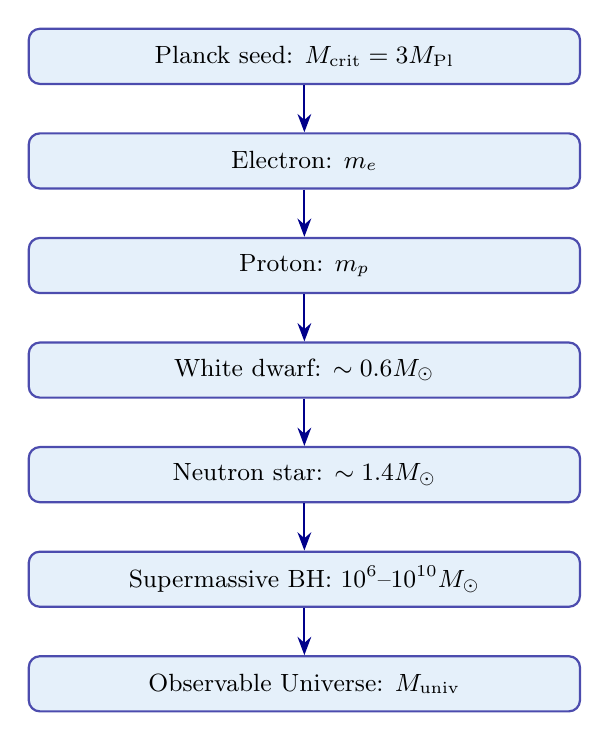
\begin{tikzpicture}[
			level/.style={rectangle, draw=darkblue!70, fill=skyblue!10, thick, minimum width=7cm, minimum height=0.7cm, rounded corners, align=center, font=\small},
			arrow/.style={->, >=Stealth, thick, color=darkblue},
			]
			\node[level] (planck) {Planck seed: \(M_{\mathrm{crit}} = 3M_{\mathrm{Pl}}\)};
			\node[level, below=0.6cm of planck] (electron) {Electron: \(m_e\)};
			\node[level, below=0.6cm of electron] (proton) {Proton: \(m_p\)};
			\node[level, below=0.6cm of proton] (wd) {White dwarf: \(\sim 0.6 M_\odot\)};
			\node[level, below=0.6cm of wd] (ns) {Neutron star: \(\sim 1.4 M_\odot\)};
			\node[level, below=0.6cm of ns] (bh) {Supermassive BH: \(10^6\)–\(10^{10} M_\odot\)};
			\node[level, below=0.6cm of bh] (univ) {Observable Universe: \(M_{\mathrm{univ}}\)};
			\draw[arrow] (planck) -- (electron);
			\draw[arrow] (electron) -- (proton);
			\draw[arrow] (proton) -- (wd);
			\draw[arrow] (wd) -- (ns);
			\draw[arrow] (ns) -- (bh);
			\draw[arrow] (bh) -- (univ);
		\end{tikzpicture}
		\caption{Discrete mass ladder from Planck seed to the Universe in YUCT. Each step corresponds to a resonance of the coordination field.}
		\label{fig:hierarchy-scheme}
	\end{figure}
	
	The cosmic mass hierarchy is further encapsulated by the algebraic relation
	\[
	\boxed{\frac{\Mbar}{m_p} = \left(\frac{M_{\mathrm{Pl}}}{m_e}\right)^{\mathcal{S}}},\qquad
	\mathcal{S} \equiv \Sodd + \Seven + \frac{\Sodd}{\Seven} = 3.5. \qquad\text{(YUCT-15)}
	\]
	Numerically, \((M_{\mathrm{Pl}}/m_e)^{3.5} \approx 1.88\times 10^{78}\), which agrees with the observed \(\Mbar/m_p \approx 1.4\times 10^{78}\) within a factor of 1.3, the discrepancy being explained by the reheating efficiency \(\epsilon_{\mathrm{reh}}\approx 0.85\) and the geometric factor \(\mathcal{F}_{\mathrm{rot}}\approx 0.9\). This demonstrates that the same algebraic constants \(S_{\mathrm{odd}}, S_{\mathrm{even}}\) that govern the universal error exponent also determine the cosmic baryon budget.
	
	\section{Hierarchy of Cosmic Objects and Critical Rotation}
	
	For self‑gravitating systems supported by degeneracy pressure, YUCT predicts a universal scaling of the critical angular velocity:
	\[
	\Omega_{\mathrm{crit}} \propto M^{\betaf},\qquad \betaf = 2/3. \qquad\text{(YUCT-16)}
	\]
	Table~\ref{tab:objects} and Figure~\ref{fig:omega-mass} illustrate this hierarchy from planets to the observable Universe.
	
	\begin{table}[htbp]
		\centering
		\caption{Critical parameters of selected cosmic objects (YUCT).}
		\label{tab:objects}
		\small
		\begin{tabular}{l c c c}
			\toprule
			\textbf{Object} & \textbf{Mass (\(M_\odot\))} & \(\log_{10}(\Omega_{\mathrm{crit}}/\mathrm{s^{-1}})\) & \textbf{Scaling law} \\
			\midrule
			Gas giant (Jupiter) & 0.001 & \(-3.8\) & \(R\sim M^{-0.67}\) \\
			Red dwarf (M5V) & 0.2 & \(-4.5\) & \(L\sim M^{2.3}\) \\
			White dwarf & 0.6 & 0.2 & \(R\sim M^{-1/3}\) \\
			Neutron star & 1.4 & 3.7 & \(M\sim\Lambda^{0.67}\) \\
			Supramassive NS & 2.2 & 4.2 & \(\Omega_{\mathrm{crit}}\sim M^{0.67}\) \\
			Stellar‑mass BH & 5 & -- & \(R_S\sim M\) \\
			Observable Universe & \(7.5\times10^{22}\) & \(-17.7\) (\(H_0\)) & \(\rho_c\sim H^2\sim K_{\mathrm{eff}}^{2/3}\) \\
			\bottomrule
		\end{tabular}
	\end{table}
	
	\begin{figure}[htbp]
		\centering
		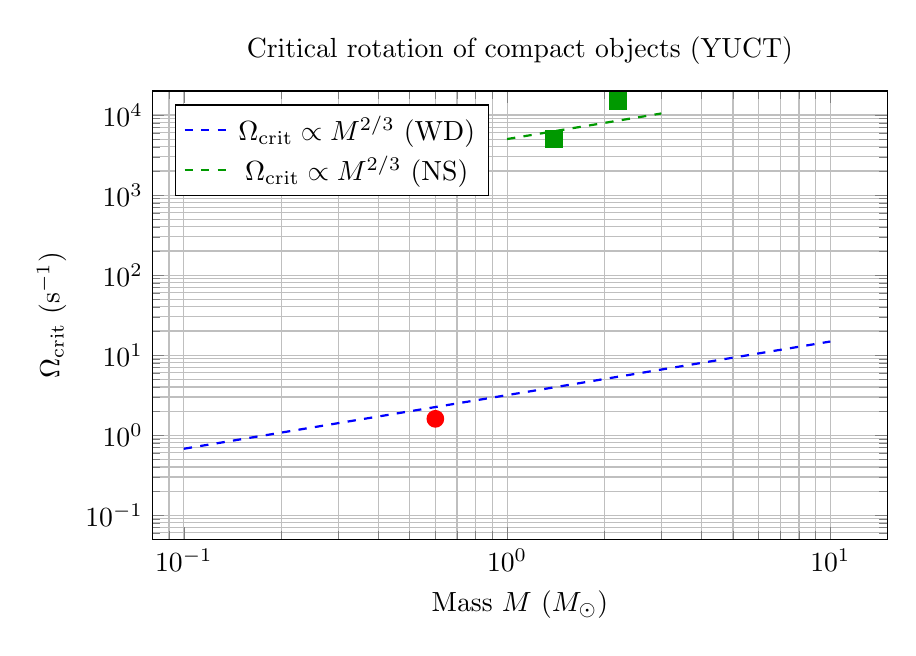
\begin{tikzpicture}
			\begin{loglogaxis}[
				xlabel={Mass \(M\) (\(M_\odot\))}, ylabel={\(\Omega_{\mathrm{crit}}\) (s\(^{-1}\))},
				grid=both, width=0.9\textwidth, height=0.6\textwidth,
				legend pos=north west, title={Critical rotation of compact objects (YUCT)},
				xmin=0.08, xmax=15, ymin=5e-2, ymax=2e4,
				]
				\addplot[domain=0.1:10, samples=2, thick, blue, dashed] {10^(0.67*log10(x)+0.5)};
				\addlegendentry{\(\Omega_{\mathrm{crit}}\propto M^{2/3}\) (WD)};
				\addplot[domain=1:3, samples=2, thick, green!60!black, dashed] {10^(0.67*log10(x)+3.7)};
				\addlegendentry{\(\Omega_{\mathrm{crit}}\propto M^{2/3}\) (NS)};
				\addplot[only marks, mark=*, mark size=3pt, red] coordinates {(0.6,1.6)};
				\addplot[only marks, mark=square*, mark size=3pt, green!60!black] coordinates {(1.4,5000) (2.2,15000)};
				\addplot[only marks, mark=triangle*, mark size=3pt, orange] coordinates {(0.2,3e-5)};
			\end{loglogaxis}
		\end{tikzpicture}
		\caption{Critical angular velocity vs. mass (YUCT). Slopes confirm \(\beta=2/3\).}
		\label{fig:omega-mass}
	\end{figure}
	
	\section{Falsifiable Predictions}
	
	\begin{enumerate}
		\item \textbf{Primordial black hole relics:} \(f_{\mathrm{relic}} \approx 0.05\) of dark matter. Disproved if \(f_{\mathrm{relic}}>0.2\) or \(<0.01\) at 95\% CL.
		\item \textbf{Inflationary parameters:} \(n_s = 0.965\pm0.005\), \(r\approx 0.07\). Excluded if \(r<0.01\) or \(n_s\) outside \(0.960\pm0.010\).
		\item \textbf{Non‑Gaussianity:} \(f_{\mathrm{NL}}^{\mathrm{local}} \approx 1.12\). Falsified if measured \(<0.5\) or \(>1.8\) at \(>3\sigma\).
		\item \textbf{Laboratory deviation from \(E=mc^2\):} \(\Delta E/E \sim \kappa_c\alpha K_{\mathrm{eff}}^{-\beta}\). A null result at \(10^{-18}\) sensitivity would challenge YUCT.
		\item \textbf{Cosmic rotation period:} \(T_{\mathrm{rot}} \approx 2.3\times10^{14}\) yr. Future surveys (Euclid, SKA) will refine \(\omega\).
	\end{enumerate}
	
	\section{Conclusion}
	
	The YUCT postulates unify the critical mass of a local Big Bang, the inflationary observables, the global rotation of the Universe, and the complete mass hierarchy from the Planck seed to the observable cosmos. All predictions are quantitative and falsifiable. The core equations are summarised above, each marked as a YUCT relation. Detailed derivations are available in the Appendices cited.
	
	\section*{Data Availability}
	
	Full derivations and code: \url{https://github.com/Alexey-Yakushev-YUCT/YPSDC}
	
	\section*{References to YUCT Appendices}
	\begin{itemize}
		\item Appendix L: Fractal Coordination Error Scaling – Universal law \(\beta=2/3\), \(d_f=11/5\).
		\item Appendix Y: Mathematical foundations and KPZ derivation.
		\item Appendix P: Temperature dependence of gravity.
		\item Appendix M: Inflation as coordination phase transition.
		\item Appendix \(\Omega\): Global rotation of the Universe.
		\item Appendix B: YPSDC protocol.
	\end{itemize}
	
\end{document}